\documentclass[border=4pt]{standalone}

\usepackage{amsmath}
\usepackage{tikz}
\usepackage{mathdots}
\usepackage{yhmath}
\usepackage{cancel}
\usepackage{color}
\usepackage{siunitx}
\usepackage{array}
\usepackage{multirow}
\usepackage{amssymb}
\usepackage{gensymb}
\usepackage{tabularx}
\usepackage{booktabs}
\usetikzlibrary{fadings}
\usetikzlibrary{patterns}


\begin{document}

\tikzset{every picture/.style={line width=0.75pt}} %set default line width to 0.75pt

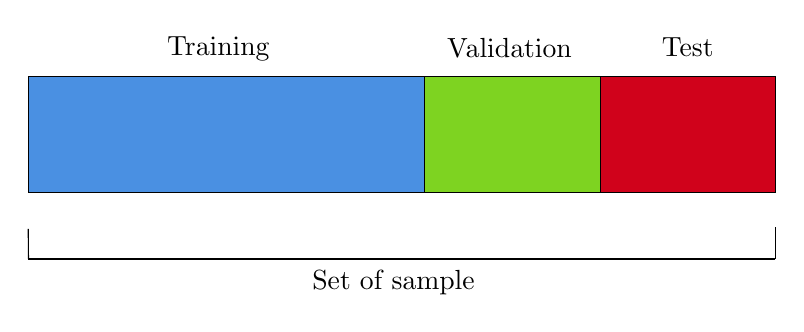
\begin{tikzpicture}[x=0.75pt,y=0.75pt,scale=0.75]%yscale=-1,xscale=1]
    %uncomment if require: \path (0,362.03123474121094); %set diagram left start at 0, and has height of 362.03123474121094

    %Shape: Rectangle [id:dp7908816581995917]
    \draw  [color={rgb, 255:red, 0; green, 0; blue, 0 }  ,draw opacity=1 ][fill={rgb, 255:red, 74; green, 144; blue, 226 }  ,fill opacity=1 ] (22,127.4) -- (276.57,127.4) -- (276.57,201.77) -- (22,201.77) -- cycle ;
    %Shape: Rectangle [id:dp3308741251015308]
    \draw  [color={rgb, 255:red, 0; green, 0; blue, 0 }  ,draw opacity=1 ][fill={rgb, 255:red, 126; green, 211; blue, 33 }  ,fill opacity=1 ] (276.57,127.4) -- (389.2,127.4) -- (389.2,201.77) -- (276.57,201.77) -- cycle ;
    %Shape: Rectangle [id:dp10818385700745736]
    \draw  [color={rgb, 255:red, 0; green, 0; blue, 0 }  ,draw opacity=1 ][fill={rgb, 255:red, 208; green, 2; blue, 27 }  ,fill opacity=1 ] (389.2,127.4) -- (501.84,127.4) -- (501.84,201.77) -- (389.2,201.77) -- cycle ;
    %Straight Lines [id:da25216151118859864]
    \draw    (22,84.63) -- (501.84,84.63) ;


    %Straight Lines [id:da7185220245845878]
    \draw    (22,84.63) -- (21.84,104.04) ;


    %Straight Lines [id:da9658692602555647]
    \draw    (501.84,84.63) -- (501.84,105.04) ;



    % Text Node
    \draw (256.5,69.5) node [align=left] {Set of sample};
    % Text Node
    \draw (144,219.5) node [align=left] {Training};
    % Text Node
    \draw (331,220.5) node [align=left] {Validation};
    % Text Node
    \draw (445.5,220.5) node [align=left] {Test};


\end{tikzpicture}

\end{document}
